\documentclass{article}

\usepackage[left=1in, right=1in, top=1in, bottom=1in]{geometry}

\usepackage{setspace}
\usepackage{fancyhdr}
\usepackage{hyperref}
\usepackage{amsthm}
\usepackage{amssymb}
\usepackage{multirow}
\usepackage{enumitem}
\usepackage{graphicx}
\usepackage{makecell}
\usepackage{booktabs}
\usepackage{titlesec}
\usepackage{amsmath}
\usepackage{pdfpages}
\usepackage{enumitem}
\usepackage{caption}


\setcounter{secnumdepth}{4}

\hypersetup{
    colorlinks=true,     
    urlcolor=magenta
}

\renewcommand{\qedsymbol}{\rule{0.7em}{0.7em}}

\newlength\tindent
\setlength{\tindent}{\parindent}
\setlength{\parindent}{0pt}
\renewcommand{\indent}{\hspace*{\tindent}}
\setlength{\parskip}{0em}

\newenvironment{blockquote}{%
  \par%
  \vskip1em
  \leftskip=2em\rightskip=2em%
  \noindent\ignorespaces}{%
  \par\vskip1em}

\newenvironment{blockquote2}{%
	\par%
	\vskip1em
	\leftskip=4em\rightskip=4em%
	\noindent\ignorespaces}{%
	\par\vskip1em}

\pagestyle{fancy}
\fancyhf{}
\fancyhead[LO]{STA5176}
\fancyhead[RO]{Kyle Ligon}
\fancyfoot[LO]{Chapter 11 and 12}
\fancyfoot[RO]{\thepage}
 
\renewcommand{\headrulewidth}{0.5pt}
\renewcommand{\footrulewidth}{0.5pt}

\begin{document}
\section*{Chapter 11 and 12 Homework}
\section*{Due 4-27-2018}
\subsection*{Data from 10.14}
\subsubsection*{a) Would it be appropriate to use a normal approximation in conducting a
statistical test of the research hypothesis that over half of persons suffering
from chronic pain are over 50 years of age?}
With $\pi(n) > 5$ and (1-$\pi)(n) > 5$, it is appropriate to use a normal approximation.  \\

\subsubsection*{b)Using the data in the survey, is there substantial evidence ($\alpha$ = 0.05) 
that more than half of persons suffering from chronic pain are over 50 years of age?}

$H_{0}: \pi$ = 0.50 \\
$H_{1}: \pi >$ 0.50 \\

Test Statistic: \\
We have a $\chi^{2}$ = 35.28 and a p-value of 1.428x$10^{-9}$

Rejection Region:
Reject if p-value is less than 0.05.  

Conclusion/Interpretation:
Since our p-value is less than 0.05, we have significant evidence to suggest reject the null hypothesis is equal to 0.50.  There appears to be evidence that the probability of success is greater than 0.50.  

\subsubsection*{c) Place a 95\% confidence interval on the proportion of persons suffering from 
chronic pain that are over 50 years of age.}
We are 95\% confident the true percent of people who would be over 50 years of age experiencing chronic pain is between 0.5711 and 0.6389.  

\subsubsection*{a) Place a 95\% confidence interval on p1-p2, the difference in the proportions of customers purchasing lawnmowers with and without the warranty. }
We are 95\% confident the true difference in percents of customers who buy warranties split between customers offered a warranty and those not offered a warranty is between 0.0001 and 0.4799.  

\subsubsection*{b) Test the research hypothesis that offering the warranty will increase the proportion of customers who will purchase a mower.  Use $\alpha$ = 0.05.}
Hypotheses: \\
$H_{0}: \pi_{Offered} = \pi_{NotOffered}$ \\
$H_{1}: \pi_{Offered} > \pi_{NotOfferec}$ \\

Test Statistic: \\ 
We have a $\chi^{2}$ of 2.4802.   \\ 

Rejection Region: \\
We reject the null hypothesis if our $\chi^{2} > \chi_{0.95, 1}^{2} = 3.841$  \\

Conclusion/Interpretation:
Since we do not have a test statistic that is bigger than our rejection region, we will not reject the null hypothesis that the proportions are the same.  We do not have enough evidence to say offering customers a warranty will lead to increases warranty purchases.  

\subsubsection*{c) Are the conditions for using a large-sample test to answer the question in part b) satisfied?  If not, apply an exact procedure.}
Since $\left(\pi_{NotOffered}\right)(25) < 5$, we have not met the requirements to use a large sample test.  We will use Fisher's Exact to look at the results.  \\

Hypotheses: \\
$H_{0}: \pi_{Offered} = \pi_{NotOffered}$ \\
$H_{1}: \pi_{Offered} > \pi_{NotOffered}$  \\

Test Statistic/P-value: \\
We have a p-value of 0.05683. \\

Rejection Region: \\
We will reject if p-value is less than 0.05 = $\alpha$.  

Conclusion/Interpretation: \\
With a p-value greater than $\alpha$, we do not have significant evidence to reject the null hypothesis that the take rates on warranties are the same.  There does not appear to be evidence that the take rate increases with an offer for a warranty.  

\subsubsection*{d) Based on your results from parts a) and b), should the dealer offer the warranty?}
The dealer should not offer the warranty.  The test stat isn't statistically significant at $\alpha$ = 0.05. 

\subsection*{10.42 (b,d)}
\subsubsection*{b) Is the promotion decision for the fireman related to the age of the fireman? Use $\alpha$ = 0.05.}
Hypotheses: \\
$H_{0}$: Promotion as a fireman is independent of age.  \\ 
$H_{1}$: Promotion as a fireman depends on age.  \\

Test Statistic:\\
We have a $\chi^{2} = 12.796$ and a p-value = 0.0051.

Rejection Region: \\
We would reject the null hypothesis if our test stat is greater than $\chi_{3, 0.95}^{2} = 7.815$ \\

Conclusion/Interpretation: \\
There is evidence to reject the null hypothesis that age doesn't impact promotion rate.  It appears the promotion of a fireman does depend on their age.  

\subsubsection*{What are some other variables, besides age that needed to be addressed in an age discrimination analysis?}
I believe sex/gender, years with the department, and number of previous promotions are adequate variables to split this data on.

\subsection*{10.43}
\subsubsection*{a) Is the age of the fireman related to whether or not the fireman is promoted?  Use $\alpha$ = 0.05.}
Hypotheses: \\
$H_{0}$ Promotion as a fireman is independent of age.  \\ 
$H_{1}$: Promotion as a fireman depends on age.  \\

Test Statistic:
We have a $\chi^{2} = 0.15549$ and a p-value = 0.6933.

Rejection Region:
We would reject the null hypothesis if our test stat is greater than $\chi_{1, 0.95}^{2} = 3.841$ \\

Conclusion/Interpretation:
Since we do not have a test stat that is bigger than our rejection region, we will not reject the null hypothesis.  There does not seem to be evidence that promotion as a fireman depends on age.  

\subsection*{b) Is your conclusion concerning age discrimination different from your conclusion using the data in Exercise 10.42?}
Yes, with a p-value greater than 0.05, it does not appear that the age group is different for promotion potential.  However, I am suspicious of lumping everyone into one group that is below 40 years of age.


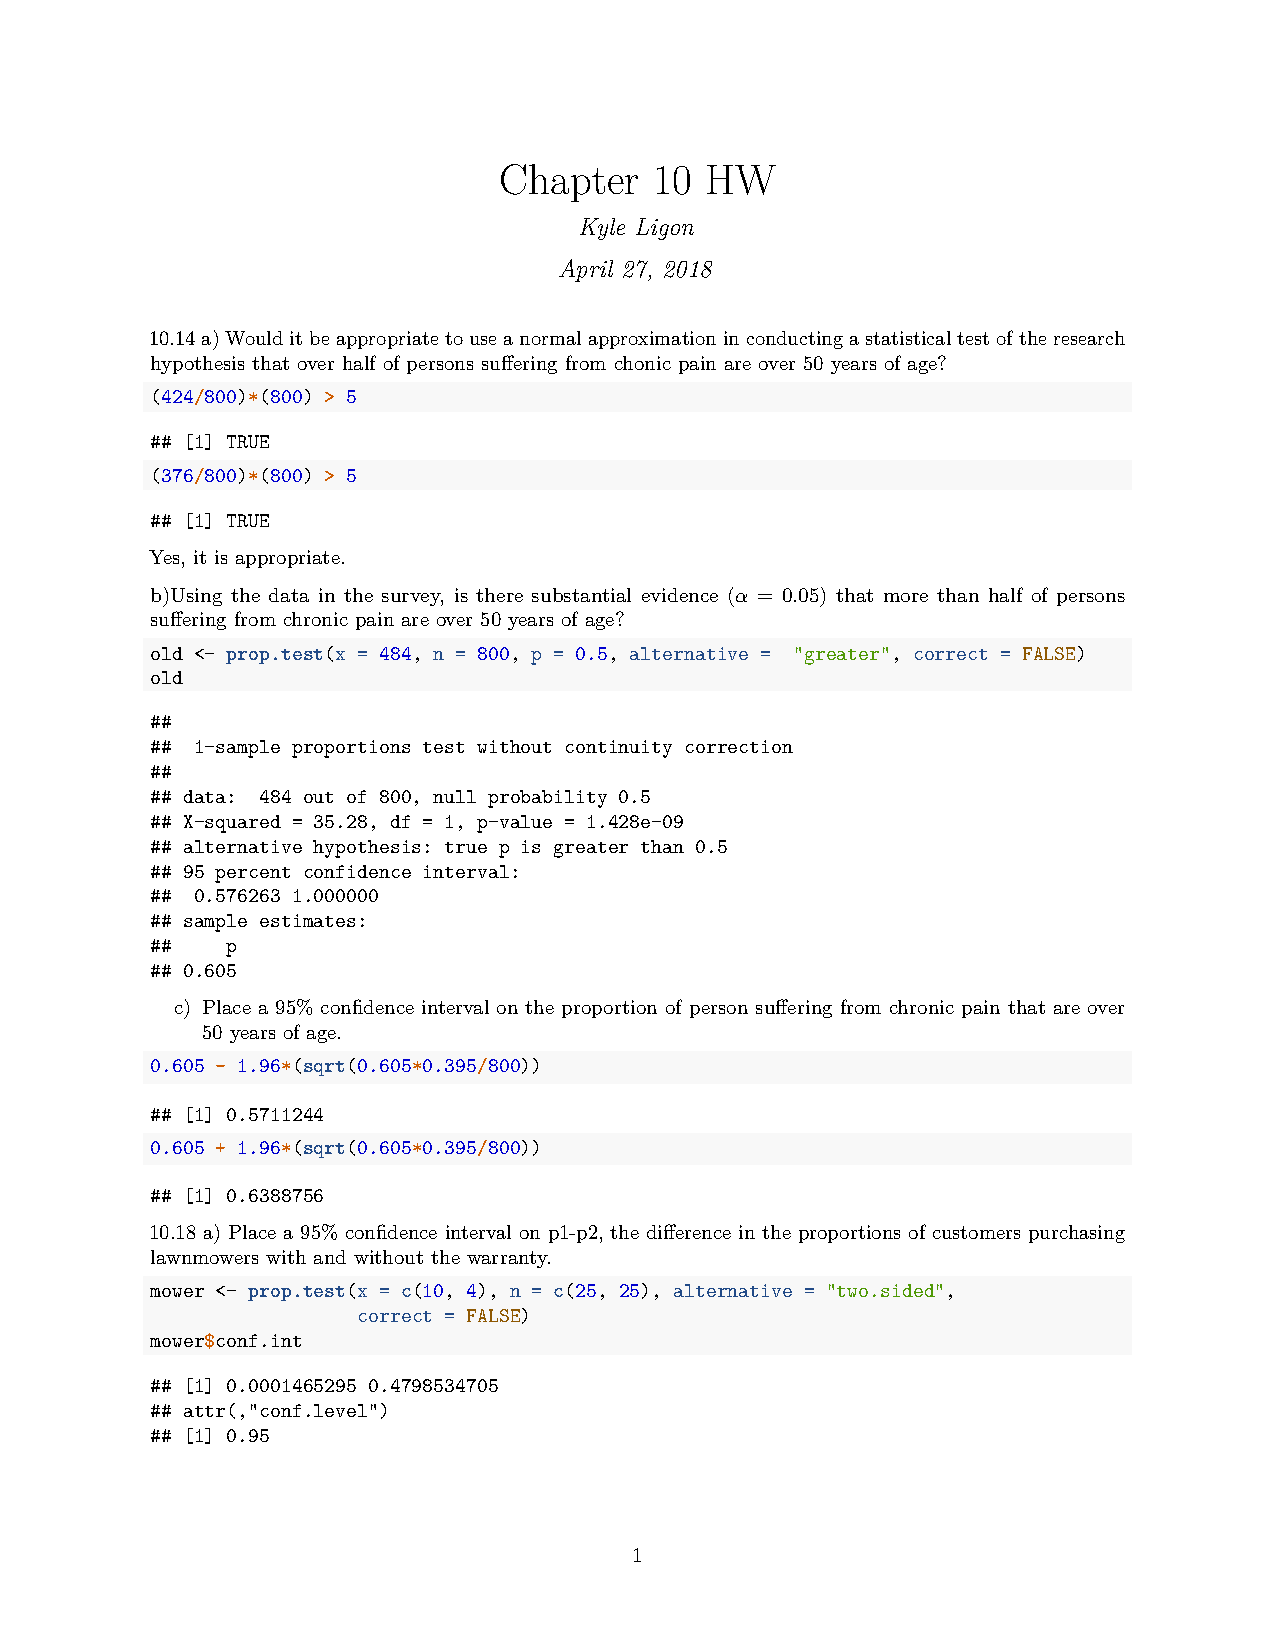
\includepdf[pages=-]{Chapter10HWR.pdf}

\end{document}